\documentclass{article}[12pt]
\usepackage{fullpage,graphicx, setspace, latexsym, cite,amsmath,amssymb,color,subfigure}
%\usepackage{epstopdf}
%\DeclareGraphicsExtensions{.pdf,.eps,.png,.jpg,.mps} 
\usepackage{amssymb} %maths
\usepackage{amsmath} %maths
\usepackage{amsthm}
\usepackage{graphicx}
\usepackage{ upgreek }
\usepackage{ dsfont }
\usepackage{listings}
\usepackage{xcolor}
 
\definecolor{codegreen}{rgb}{0,0.6,0}
\definecolor{codegray}{rgb}{0.5,0.5,0.5}
\definecolor{codepurple}{rgb}{0.58,0,0.82}
\definecolor{backcolour}{rgb}{0.95,0.95,0.92}
 
\lstdefinestyle{mystyle}{
    backgroundcolor=\color{backcolour},   
    commentstyle=\color{codegreen},
    keywordstyle=\color{magenta},
    numberstyle=\tiny\color{codegray},
    stringstyle=\color{codepurple},
    basicstyle=\ttfamily\footnotesize,
    breakatwhitespace=false,         
    breaklines=true,                 
    captionpos=b,                    
    keepspaces=true,                 
    numbers=left,                    
    numbersep=5pt,                  
    showspaces=false,                
    showstringspaces=false,
    showtabs=false,                  
    tabsize=2
}
 
\lstset{style=mystyle}
 

\bibliographystyle{unsrt}

\newtheorem{theorem}{Theorem}
\newtheorem{prop}{Proposition}
\newtheorem{corollary}{Corollary}
\newtheorem{lemma}{Lemma}
\newtheorem{defn}{Definition}
\newtheorem{ex}{Example}
\usepackage{float}

\def\R{\mathbb{R}}
\def\Eps{\mathcal{E}}
\def\E{\mathbb{E}}
\def\V{\mathbb{V}}
\def\F{\mathcal{F}}
\def\G{\mathcal{G}}
\def\H{\mathcal{H}}
\def\S{\mathcal{S}}
\def\P{\mathbb{P}}
\def\1{\mathbf{1}}
\def\n{\nappa}
\def\h{\mathbf{w}}
\def\v{\mathbf{v}}
\def\x{\mathbf{x}}
\def\X{\mathcal{X}}
\def\Y{\mathcal{Y}}
\def\eps{\epsilon}
\def\y{\mathbf{y}}
\def\e{\mathbf{e}}
\newcommand{\norm}[1]{\left|\left|#1\right|\right|}
\DeclareMathOperator*{\argmin}{arg\,min}
\DeclareMathOperator*{\argmax}{arg\,max}

\newcommand{\lecture}[4]{
   \pagestyle{myheadings}
   \thispagestyle{plain}
   \newpage
   % \setcounter{lecnum}{#1}
   \setcounter{page}{1}
   \setlength{\headsep}{10mm}
   \noindent
   \begin{center}
   \framebox{
      \vbox{\vspace{2mm}
    \hbox to 6.28in { {\bf ESE 680-004: Learning and Control
   \hfill Fall 2019} }
       \vspace{4mm}
       \hbox to 6.28in { {\Large \hfill Lecture #1: #2  \hfill} }
       \vspace{2mm}
       \hbox to 6.28in { {\it Lecturer: #3 \hfill Scribes: #4} }
      \vspace{2mm}}
   }
   \end{center}
   \markboth{Lecture #1: #2}{Lecture #1: #2}

   \noindent{\bf Disclaimer}: {\it These notes have not been subjected to the
   usual scrutiny reserved for formal publications. }
   \vspace*{4mm}
}

%notation

\def \E{\mathbb E}
\def \P{\mathbb P}
\def \R{\mathbb R}
\def \A{\cal A}

\begin{document}

\lecture{8}{A Whirlwind Tour of Robust Control 2}{Nikolai Matni}{Kendall J. Queen}
% Helpful Links: https://nikolaimatni.github.io/courses/ese680-fall2019/index.html
% https://courses.cs.washington.edu/courses/cse599i/18wi/

\noindent This script is the second iteration of instruction on Robust Control with an introduction into structured uncertainty. This document will focus exclusively on the small gain theorem, structured singular value, KYP Lemma, and integral quadratic constraints (IQCs). 

\section{Introduction}

This is a continuation of the discussion on robust stability. We start with a generalized plant seen in Figure \ref{initial_sys}. This plant is built to have two outputs, controlled and measured, denoted properly below in equations \ref{cont_out_eq} and \ref{meas_out_eq} respectively.   

\begin{equation}
    x_{t+1} = Ax_t + B_1w_t + B_2u_t \ \ \ 
    \caption{State}
    \label{State_eq}
\end{equation}

\begin{equation}
    z_t = C_1x_t + D_{12}u_t \ \ \ 
    \caption{Controlled \ Output}
    \label{cont_out_eq}
\end{equation}

\begin{equation}
    y_t = C_2x_t + D_{21}u_t \ \ \ 
    \caption{Measured\  Output}
    \label{meas_out_eq}
\end{equation}



\begin{equation}
    P_{ij}= C_i (zI - A)^{-1} B_j + D_{ij}
\end{equation}

\begin{figure}[h]
    \centering
    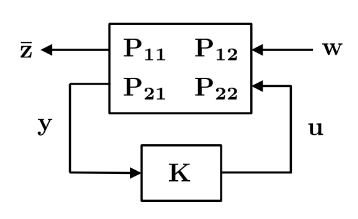
\includegraphics[width=.5\linewidth]{images/main_system.png}
    \caption{System $P$ with a feedback controller $K$.}
    \label{initial_sys}
\end{figure}

\noindent If we take our generalized plant and refer to it as system $M$ and place it in a feedback loop with some uncertainty $\Delta$, which is bounded but stable, we have a new system visualized in Figure \ref{simple_full_sys}.
This is the Linear Fractional Transform (LTF) representation of uncertainty.
This connection is robustly well-connected if $(I-M_{11} \Delta)^{-1}$ exists for all $\Delta$ $\in$ $D$. As defined in class, robust well-connectedness is synonymous with robust stability.
Furthermore, we proved that robust stability exists if and only if  $I-M\Delta$  is non-singular for all $\Delta$ $\in$ $\Delta_a$.

\begin{figure}[h]
    \centering
    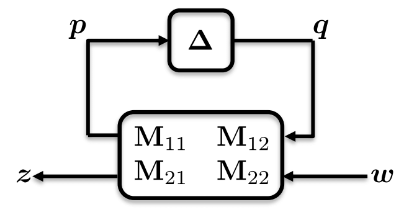
\includegraphics[width=.5\linewidth]{images/simple_full_sys.png}
    \caption{Linear Fractional Transform representation of uncertainty where $M$ is the generalized plant discussed earlier in a feedback loop with uncertainty set $\Delta$.}
    \label{simple_full_sys}
\end{figure}

\section{Small Gain Theorem}

\begin{theorem} Let \boldsymbol{Q} be a bounded linear operator, $\|\boldsymbol{Q}\|_{H_\infty}$  \textless $\infty$, and let \boldsymbol{D} = \{\mathds{\Delta} := ${\Delta : ||\Delta ||_{H_\infty} \leq 1}$\}. Then $I-Q\Delta$ is non-singular for all $\Delta \in$ \boldsymbol{D} if and only if  $\|\boldsymbol{Q}\|_{H_\infty}$ \textless 1.
\end{theorem}

\noindent In order for the Small Gain Theorem to apply there are 2 key properties that must hold. 
\begin{enumerate}
    \item Assume $M$ is stable \(||M|| _{H _\infty} < \infty\)
    
    \item \(|| \cdot||_{H_\infty} \) is a sub-multiplicative norm needed to establish that the vector space of bounded linear operators equipped with \(|| \cdot||_{H_\infty} \) norm forms a Banach Algebra. 
\end{enumerate}

\noindent Key property 2 allows us to take limits and guarantee existence. 
In the traditional sense, we would assume two stable systems $M$ and $\Delta$ are connected via feedback loop as seen in Figure \ref{simple_full_sys}. We also assume that we know these systems in regards to gain.

\begin{proof}

If: To prove the if direction, we first look at the small gain. At first glance we can apply the multiplicative property and bound $||\boldsymbol{Q} \Delta||$ as seen in equation \ref{multiplicative}. We know that $||\boldsymbol{Q}||_{H_\infty}$ \textless 1 and $||\Delta|| \leq 1$ by assumption. Therefore, we can simply deduct  equation \ref{multiplicative_end}.

If $||\boldsymbol{Q}||_{H_\infty} < 1$,
\begin{equation}
    ||\boldsymbol{Q} \Delta|| \leq ||\boldsymbol{Q}|| \cdot ||\Delta||
    \label{multiplicative}
\end{equation}

\begin{equation}
    ||\boldsymbol{Q} \Delta|| \leq ||\boldsymbol{Q}|| \cdot ||\Delta|| < 1
    \label{multiplicative_end}
\end{equation}
With this deduction, we can explicitly construct the $(I-Q\Delta)^{-1}$. Express $(I-Q\Delta)^{-1}$ as a geometric series, seen in equation \ref{geo} then prove that this series converges and exists through the triangle inequality and our previous deduction. 

\begin{equation}
    (I-Q\Delta)^{-1} = \sum_{t=0}^\infty (\boldsymbol{Q}\Delta)^t
    \label{geo}
\end{equation}
\begin{equation}
    ||\sum_{t=0}^T (\boldsymbol{Q}\Delta)^t||_{H_\infty} \leq \sum_{t=0}^T ||(\boldsymbol{Q}\Delta)^t||_{H_\infty} \leq \sum_{t=0}^T ||\boldsymbol{Q}\Delta||^t_{H_\infty}
    \label{Triangle_ineq}
\end{equation}
Equation \ref{Triangle_ineq} shows the use of the triangle inequality. We then can simply apply the solution we know for the geometric series as the limit approaches $\infty$, seen in equation \ref{geo_series}  . 

\begin{equation}
    \label{geo_series}
    \lim_{x\to\infty} \sum_{t=0}^T ||\boldsymbol{Q}\Delta||^t_{H_\infty} = \frac{1}{1-||\boldsymbol{Q}\Delta||}
\end{equation}

\noindent Only if: If $||\boldsymbol{Q}|| \geq 1$, construct a $\Delta$, where $||\Delta|| \leq 1$, such that $I-\boldsymbol{Q}\Delta$ is singular. We start with the observation in equation \ref{init_obs}. Normally, the spectral norm of a matrix would equal that of its transpose but in this case it is conjugate tranpose due to \boldsymbol{Q}'s  complex values. Now forward, we will refer to $\lambda_{max}(\boldsymbol{QQ}^*)$ as $\lambda$. 

\begin{equation}
    \label{init_obs}
    || \boldsymbol{Q}||^2_{H_\infty} = || \boldsymbol{Q}^*||^2_{H_\infty} = \lambda_{max}(\boldsymbol{QQ}^*) \geq 1
\end{equation}

\noindent Through the definition of an eigenvalue, we know that $\lambda I - \boldsymbol{QQ}^*$ is singular. $\lambda \neq 0$ which allows the scaling operation in equation \ref{eig_div} and does not change its singular status. 

\begin{equation}
\label{eig_div}
    \frac{1}{\lambda} \cdot (\lambda I - \boldsymbol{QQ}^*) = I - \frac{\boldsymbol{QQ}^*}{\lambda}
\end{equation}
\noindent By writing equation \ref{eig_div} using our definition of $\lambda$, we produce equation \ref{lam_replace} and claim that $\Delta :=\frac{\boldsymbol{Q}^*}{||\boldsymbol{Q}^*||_{H_\infty}^2}$. Then we apply the $H_\infty$ norm to $
\Delta$ in equation \ref{delt_fin} which completes the construction of our counter example.

\begin{equation}
    I - \frac{\boldsymbol{QQ}^*}{||\boldsymbol{Q}^*||^2_{H_\infty}}
    \label{lam_replace}
\end{equation}
\begin{equation}
    \label{delt_fin}
    ||\Delta||_{H_\infty} = \frac{||\boldsymbol{Q}^*||_{H_\infty}}{||\boldsymbol{Q}^*||^2_{H_\infty}} =  \frac{1}{||\boldsymbol{Q}^*||_{H_\infty}} \leq 1
\end{equation}

\noindent Therefore, through this proof we have shown that the condition is both necessary and sufficient. 
\end{proof}









\section{Scaled Small Gain Test}
%Scaled small gain test for block diagonal (but otherwise unstructured) bounded uncertainty.

Small gain is a sufficient but a conservative bound. When working with a block diagonal, defined in equation \ref{block_diagonal}, $||\boldsymbol{M}|| \geq 1$ holds no weight and does not really imply anything. More specifically it does not imply that $I-\boldsymbol{M}\Delta$ is singular for some uncertainty in $\boldsymbol{\Delta}_a$. In order to scale things we use a trick that involves the use of a commutant set, introduced in equation \ref{comm_set}.

\begin{equation}
    \label{block_diagonal}
    \boldsymbol{\Delta}_a = {\boldsymbol{\Delta} : ||\boldsymbol{\Delta}|| \leq 1, \boldsymbol{\Delta} = blkdiag(\boldsymbol{\Delta}_1,\boldsymbol{\Delta}_2, \ldots, \boldsymbol{\Delta}_d}
\end{equation}

\begin{equation}
    \label{comm_set}
    \mathcal{G} = {\boldsymbol{\Gamma} : \Gamma\boldsymbol{\Delta} = \boldsymbol{\Delta}\Gamma, \: \Gamma^{-1} \: exists}
\end{equation}

\noindent The commutant set is the set of operators that commutes with any $\Delta$ within the block diagonal, $\boldsymbol{\Delta}_a$, of uncertainty. With the commutant set we plan to prove that $I-\boldsymbol{M}\Delta$ is singular.



\subsection{Proof of Small Gain Test with Block}
% Proof of (a) the commutant set being as described on slide 28 -30 look at the notes and video

Due to the fact that inverse, $\Gamma^{-1}$, shares the same communtant properties we can rewrite $I-\boldsymbol{M}\Delta$, seen in equation \ref{comm_trick}. This provides us now with a scaled small gain, now slightly altering our proof. Now $I-\boldsymbol{M}\Delta$ is non-singular if and only if $I-\Gamma\boldsymbol{M}\Gamma^{-1}\Delta$ is non-singular. 
If there exists a $\Gamma$ such that $||\Gamma \boldsymbol{M}\Gamma^{-1}|| < 1$ then the system is robustly well-connected.

\begin{equation}
    \label{comm_trick}
    \Gamma(I-\boldsymbol{M}\Delta)\Gamma^{-1} = I-\Gamma\boldsymbol{M}\Delta\Gamma^{-1} = I-\Gamma\boldsymbol{M}\Gamma^{-1}\Delta
\end{equation}

\noindent The proof is the same operational steps as the small gain proof seen above in Section 2.
\section{Kalman-Yakubovich-Popov (KYP) Lemma }
% First state the KYP Lemma as in Theorem 2 of https://www-sciencedirect-com.proxy.library.upenn.edu/science/article/pii/0167691195000631, and show how it reduces to what we have on slide 30 by choosing M = [C’; D’][C,D], and prove the sufficient direction (and cite Rantzer for necessary direction).
One of the most fundamental tools in systems theory is the Kalman-Yakubovich-Popov (KYP) Lemma. In short, Popov introduced a criterion that gave a frequency condition for stability of a feedback system with a memoryless nonlinearity. In respect to the previous examples, KYP is applied to our feedback uncertainty system and provided a computational test.
\begin{theorem}\footnote{\cite{RANTZER19967}}
Give $A$, $B$, $M$, with $det(e^{j\omega} I - A) \neq 0)$ for $\omega  \in \mathbb{R}$ and (A,B) controllable, the following two statements are equivalent:
\begin{enumerate}
    \item  
    $\begin{bmatrix}
        (e^{j\omega}I - A)^{-1}B \\
        I
    \end{bmatrix}^{*} M
    \begin{bmatrix}
        (e^{j\omega}I - A)^{-1}B \\
        I
    \end{bmatrix} \leq 0 \: \forall \omega \in \mathbb{R}$.
    
    \item There exists a matrix $P \in \mathbb{R}^{nxn}$ such that $P = P^T$ and
    $M + 
    \begin{bmatrix}
        A^{T}PA - P & A^T PB \\
         B^{T}PA & B^T PB
    \end{bmatrix} \leq 0.
    $
    The corresponding equivalence for strict inequalities holds even if (A,B) is not controllable.
    \end{enumerate}
\end{theorem}
\noindent At this point, we will prove the sufficiency direction for KYP, where the linear matrix inequality (LMI) implies the norm condition. 

\begin{proof}
Suppose there exists a $P$ that satisfies the LMI given above. We want to show that the LMI implies the norm condition on the system. The full LMI, equation \ref{full_LMI}, as it pertains to \boldsymbol{M}(z) = $C(zI-A)^{-1} B+D$, which is a stable, bounded linear time invariant (LTI) operator. \boldsymbol{M} = $\begin{bmatrix}
        C \\
        D
    \end{bmatrix} \cdot 
    \begin{bmatrix}
        C & D
    \end{bmatrix}$.
We then pre and post multiply the LMI. 
    
    \begin{equation}
        \label{full_LMI}
        \begin{bmatrix}
        x_t^T & w_t^T
        \end{bmatrix}
        \left( \begin{bmatrix}
        C \\
        D
    \end{bmatrix} \cdot \begin{bmatrix}
        C & D
    \end{bmatrix} +
        \begin{bmatrix}
        A^{T}PA - P & A^T PB \\
         B^{T}PA & B^T PB
    \end{bmatrix} \right) 
    \begin{bmatrix}
        x_t \\
        w_t
        \end{bmatrix} \leq 0
    \end{equation}
    
\noindent After some strategic multiplication and defining our measured output below, equations \ref{next_state} and \ref{output},  we can rewrite our LMI as in equations \ref{final_lmi}, \ref{final_lmi2}, and \ref{final_lmi3}.
\begin{equation}
    \label{next_state}
    x_{t+1} = Ax_t+Bw_t , x_0 = 0
\end{equation}

\begin{equation}
    \label{output}
    z_{t} = Cx_t+Dw_t
\end{equation}


\begin{equation}
    \label{final_lmi}
    (Ax_t+Bw_t)^T P (Ax_t+Bw_t) - x_t^T P x_t + (Cx_t+Dw_t)^T(Cx_t+Dw_t) - w_t^T w_t \leq 0
\end{equation}

\begin{equation}
    \label{final_lmi2}
    x_{t+1}^T P x_{t+1} - x_t^T P x_t + z_t^Tz_t < w_t^T w_t 
\end{equation}

\begin{equation}
    \label{final_lmi3}
    x_{t+1}^T P x_{t+1} - x_t^T P x_t + ||z_t||^2_2 < ||w_t||^2_2 
\end{equation}

\noindent This becomes a telescoping sum seen in equation \ref{telescope} and $ x_0^T P x_0$ goes to 0 per the definition in equation \ref{next_state}. Then taking the limit as $t \to \infty$ of equation \ref{telescope} we get equation \ref{tele_2}, which leads us into the norm condition as previously described. 

\begin{equation}
\label{telescope}
    \sum_{t=0}^T ||z_t||_2^2 + x_{t+1}^T P x_{t+1} - x_0^T P x_0 < \sum_{t=0}^T ||w_t||^2_2  
\end{equation}

\begin{equation}
    \label{tele_2}
    \lim_{t\to\infty} \sum_{t=0}^T ||z_t||_2^2 + x_{t+1}^T P x_{t+1} - x_0^T P x_0 < \sum_{t=0}^T ||w_t||^2_2 \\= ||z||^2_{l_2} < ||w||^2_{l_2} = \frac{||\boldsymbol{M}w||^2_{l_2}}{||w||^2_{l_2}} < 1, \: \: \forall w,t,l_2 
\end{equation}

\end{proof}
\noindent I will point you to \cite{RANTZER19967} for the proof of the sufficient direction, as it is difficult and complicated.

\subsection{Structured Uncertainty Proposition, Proposition 8.26}
% Page 273 in http://read.pudn.com/downloads143/ebook/625700/A%20Course%20In%20Robust%20Control%20Theory.pdf
% Also refer to the slides (this is a more complete version of the Proposition on slide 29 of the notes.  The only modification is that we work in discrete time, whereas they work in continuous time, the only difference is in the form of the resulting LMI, but should be clear how to adapt using the discrete time KYP Lemma).
Suppose $\boldsymbol{M}(z) = C(zI - A)^{-1}B + D$ is a stable, bounded LTI operator. Then the following are equivalent:
\begin{enumerate}
    \item There exists $\Gamma \in \mathcal{G}$ such that $||\Gamma \boldsymbol{M} \Gamma^{-1}|| < 1$.
    
    \item There exists $\Gamma \in \mathcal{G}$ such that $\Gamma$ is real and positive such that $||\Gamma^{\frac{1}{2}} \boldsymbol{M} \Gamma^{\frac{-1}{2}}|| < 1$
    
    \item There exists $P > 0$ and $\Gamma \in \mathcal{G}$, $\Gamma$ is real and positive, such that \\
    $\begin{bmatrix}
        A^{T}PA - P & A^T PB \\
         B^{T}PA & B^T PB - \Gamma
    \end{bmatrix} + 
    \begin{bmatrix}
    C^T \\
    D^T
    \end{bmatrix} \Gamma
    \begin{bmatrix}
    C & D
    \end{bmatrix} < 0
    $
\end{enumerate}
Due to their equivalence, proving one of the pieces of the proposition will hold true for the rest of them. Thereby, I will select the second condition to manipulate. Equation \ref{scaling} below is an expansion of M and shows that $B$, $C$, and $D$ will be scaled by the $\Gamma^{\frac{1}{2}}$ and $\Gamma^{\frac{-1}{2}}$ terms. Then we take the those scaled terms and plug them into a structure similar to equation \ref{full_LMI} with pre multiplication of \begin{bmatrix}
    I & 0\\
    0 & \Gamma^{\frac{1}{2}}
    \end{bmatrix} and post multiplication of
    \begin{bmatrix}
    I & 0\\
    0 & \Gamma^{\frac{1}{2}}
    \end{bmatrix}. This is expounded in equation \ref{PP_mult}.


\begin{equation}
    \label{scaling}
    \Gamma^{\frac{1}{2}} M \Gamma ^{\frac{-1}{2}} = \Gamma^{\frac{1}{2}} C (zI-A)^{-1} B \Gamma^{\frac{-1}{2}} + \Gamma^{\frac{1}{2}}D\Gamma^{\frac{-1}{2}}
\end{equation}

\begin{equation}
    \label{PP_mult}
        \begin{bmatrix}
    I & 0\\
    0 & \Gamma^{\frac{1}{2}}
    \end{bmatrix}
        \begin{bmatrix}
        x_t^T & w_t^T
        \end{bmatrix}
        \left( \begin{bmatrix}
        C \\
        D
    \end{bmatrix} \cdot \begin{bmatrix}
        C & D
    \end{bmatrix} +
        \begin{bmatrix}
        A^{T}PA - P & A^T PB \\
         B^{T}PA & B^T PB
    \end{bmatrix} \right) 
    \begin{bmatrix}
        x_t \\
        w_t
        \end{bmatrix} 
         \begin{bmatrix}
    I & 0\\
    0 & \Gamma^{\frac{1}{2}}
    \end{bmatrix} \leq 0    
\end{equation}

\noindent Since we know that the setup from equation \ref{full_LMI} is a positive definite matrix which is being sandwiched by symmetric positive matrices, we can assume that the conditions do not change. This then refers back to the idea  of a scaled small gain test previously discussed in Section 3. 



\section{Structured Singular Value}
% Simply define what the structured singular value is, and give examples of different uncertainty sets and why you would use them (as on slide 32.). Section 8.3 of the above linked pdf may come in handy.
% Strongly influenced - https://www.youtube.com/watch?v=yzUb2yYTkkc&feature=youtu.be
The Structured singular value addresses the a problem where there is more structure in the uncertainty of the system. In the slides, we spoke about scalar and matrix uncertainties with restrictions which would apply the idea of a structure singular value. This is necessary because even with a small gain or scaled small gain test is still very conservative in bounding. 

\begin{defn}
Given an uncertainty set $\emph{\boldsymbol{\Delta}}$, the structured singular value of an operator \boldsymbol{M} is 

\[ \mu(\boldsymbol{M}, \emph{\boldsymbol{\Delta}}) := \frac{1}{inf\{||\Delta|| : \:  \Delta \in \emph{\boldsymbol{\Delta}} \: and \: (I-\Delta \boldsymbol{M})is \: singular \} } \],

if the infinmum is finite or defined. Otherwise $\mu(\boldsymbol{M, \emph{\boldsymbol{\Delta}}}) = 0$. 
\end{defn}

\noindent The structured singular value can be applied to structured uncertainty examples such as the following. 

\begin{enumerate}
    \item Single Uncertainty: $\emph{\boldsymbol{\Delta}}_s  = \big \{ \delta I: \delta \in \mathcal{C}, \: 0 < |\delta| \leq 1\big \}$
    
    
    \item Block Diagonal Uncertainty: $\boldsymbol{\Delta} \in \mathcal{C}^{nxn}: \: \boldsymbol{\Delta} = \begin{bmatrix}
    \boldsymbol{\Delta}_{1} & & 0 \\
    & \ddots & \\
    0 & & \boldsymbol{\Delta}_{r}
  \end{bmatrix}$
    
    
\end{enumerate}

\noindent I use $\emph{\boldsymbol{\Delta}}$ to define a certainty set in the above equations. In item 1, we see an uncertainty set where the diagonal element, $\delta I$, is a one singular value between 0 and 1. This makes the computation of the structured singular value pretty straightforward. 

\[|| \emph{\boldsymbol{\Delta}}|| = \sigma_{max}(\emph{\boldsymbol{\Delta}}) = |\delta| \leq 1 \: for \:all \: \emph{\boldsymbol{\Delta}} \in \emph{\boldsymbol{\Delta}}_s \]

\noindent In words, we are saying that any uncertainty constrained to the set of $\emph{\boldsymbol{\Delta}}_s$ then we can find the eigenvalue, $\lambda$ of operator \boldsymbol{M}. 

\[|I - A\emph{\boldsymbol{\Delta}}| = |I-\delta \boldsymbol{M}| = 0 = \delta | \delta^{-1} I - \boldsymbol{M}| \]
We then set the eigenvalue $\lambda$ = $\delta^{-1}$ and find the new solution below. This proves that $\lambda$ is an eigenvalue of \boldsymbol{M} by the eigenvalue equation. 

\[ |\lambda I - \boldsymbol{M}| = 0 \]

\noindent This also raised the question of bounds for $\delta$ and why it cannot be 0. If $\delta = 0$ then it would invalidate the first step, making the determinant, $|I-\delta \boldsymbol{M}|$, = 1.

\noindent The second example is dealing with a an uncertainty set that is a matrix of blocks, $\emph{\boldsymbol{\Delta}}_x$, that each of a scalars along the diagonals as $\emph{\boldsymbol{\Delta}}_i =  \delta_i I$. If you could imagine, this process has the same cruxes as the first example you just have to proceed for every block in the uncertainty set. 

\noindent In general it is about NP-hard to compute the structured singular value, but it is very well-studied. In addition, good computationally tractable upper and lower bounds exist to better understand the 


\subsection{S Procedure}
% S-procedure: introduce the lossless and lossy S-procedures, as introduced in the notes: only prove the sufficiency (easy direction).  Emphasize the notion of constraint qualification needed for necessary and sufficiency of conditions.  Apply lossless S-procedure to the example that we saw in class.  These slides should be useful https://stanford.edu/class/ee363/lectures/lmi-s-proc.pdf.
The S-procedure is used when your uncertainty is not linear, exemplified in equation \ref{IQC_example} where we would want to prove stability. In this case, we would use the Lyapunov function, $V(x) = x^TPx, \: P > 0$, to prove stability. Note the lipschitz bound placed on $||g(x_t)||$.
\begin{equation}
    \label{IQC_example}
    x_{t+1} = Ax_t + g(x_t), \: ||g(x_t)||_2 \leq \gamma ||x_t||_2
\end{equation}
More specifically we would need $V(x_{t+1}) - V(x_{t}) \leq -\eps V(x_t)$. Equation \ref{IQC_example} shows the difference between our next state and current state cannot be any larger than some scaled version of the current state, where $\eps > 0$. This is a condition necessary for exponential stability for some $\eps > 0$. This can be equivalently written in the form in equations \ref{init_example} and \ref{full_example} by plugging in the dynamics and manipulating the inequality. Note the substitution of $g(x_t)=z_t$.

\begin{equation}
    \label{init_example}
    (A x_t + z_t)^T P (A x_t + z_t) - x_t^T P x_t < -\eps(x_t^T P x_t) , \: \: \forall t \: where \: z_t = g(x_t) 
\end{equation}

\begin{equation}
 \label{full_example}
    (A x_t + z_t)^T P (A x_t + z_t) - x_t^T P x_t +\eps(x_t^T P x_t) < 0 \Rightarrow  (A x_t + z_t)^T P (A x_t + z_t) (1-\eps) x_t^T P x_t < 0
\end{equation}
    
    
    
\begin{equation}
    \label{further_flush}
    \begin{bmatrix}
    x_t \\ z_t
    \end{bmatrix}^T 
    \begin{bmatrix}
        A^{T}PA - (1-\eps)P & A^T P \\
         PA &P
    \end{bmatrix}  
    \begin{bmatrix}
    x_t \\
    z_t
    \end{bmatrix}
    \leq 0
\end{equation}
Equation \ref{further_flush} shows a matrix representation of equation \ref{full_example}. Notice the pre and post multiply that is similar to what we see in the KYP Lemma in Section 4. At this point, we would only need to find a P that satisfies the inequality $P > 0$. By renaming the inequality in equation \ref{further_flush} as \boldsymbol{*}, we need to find $P>0$ such that (\boldsymbol{*}) $\forall z_t = g(x_t)$. In order to encode this information we can rewrite as seen in equation \ref{encoding}.

\begin{equation}
    \label{encoding}
    \begin{bmatrix}
    x \\ z
    \end{bmatrix}^T 
    \begin{bmatrix}
        \gamma^2 I & 0 \\
         0 &-I
    \end{bmatrix}  
    \begin{bmatrix}
    x \\
    z
    \end{bmatrix}
    \geq 0
    \Rightarrow
    \gamma^2 ||x||^2 \geq ||z||^2
\end{equation}
Equation \ref{encoding} enforces that if z is produced by g(x), which satisfies the lipschitz bound, then the inequality \boldsymbol{*} is also satisfied. The use of the S-procedure allows us to prove that this holds true.


\noindent In an abstract sense, $v^T F_1 v \geq 0 $ \Rightarrow $v^T F_0 v \geq 0$, where $F_i = F_i^T$. When referring to the problem stated above, $v^T F_1 v \geq 0 $ is a reference to the constraint, lipschitz bound, from above and $v^T F_0 v \geq 0$ is the stability constraint, which is implied from the constraint.

\noindent To prove the sufficient condition:  


\begin{proof}
$\exists \tau \geq 0$ such that $F_0 \geq \tau F_1$, in the positive semi-definite sense.
\begin{equation}
    z^T F_1 z \geq 0 \Rightarrow z^T F_0 z \geq \tau z^T F_1 z \geq 0
\end{equation}
\end{proof}

\noindent This is a necessary and an exact condition. The necessary direction is very hard to prove, but can be raised through proving if $\exists u $ such that $u^T F_1 u > 0$.

\subsection{Lossless S-Procedure}
In reference to the example presented in Section 5.1, specifically equation \ref{further_flush}, if we set $\eps = 0$, we would have $v^T F_1 v \geq 0 $, where $v \neq 0$, which implies $v^T F_0 v > 0$. This would bring us to the same result where the implication is true if and only if $F_0 > \tau F_1$ as long as the constraint qualification, $\exists u $ such that $u^T F_1 u > 0$, holds. We refer to this as a lossless S-procedure. 

\noindent Therefore to complete our example and link our bounds and stability constraint we proceed as below.

True if and only if $\exists \tau \geq 0$ and $P>0$ such that

\begin{equation}
    \tau
    \begin{bmatrix}
        \gamma^2 I & 0 \\
         0 &-I
    \end{bmatrix} +
    \begin{bmatrix}
        A^{T}PA - (1-\eps)P & A^T P \\
         PA &P
    \end{bmatrix}  <
    0
\end{equation}

\subsection{Lossy S-Procedure}
The Lossy S-procedure is best exemplified when dealing with multiple quadratic forms. For example, we let $F_0,...,F_k$ be symmetric matrices and we want a sufficient condition such that  $v^T F_1 v > 0, \: ... \: , v^T F_k v > 0 $ \Rightarrow $v^T F_0 v \geq 0$. This condition brings up the question of when does nonnegativity of a set of quadratic forms imply nonnegativity of another set. A simple sufficient condition for this is to suppose there are $\tau_1, ..., \tau_k \geq 0$, with $F_0 \geq \tau_1 F_1+...+\tau_k F_k$.  This solidifies our original sufficient condition, with no necessary conditions known, meaning that more assumption are needed but lossless versions do exist. This is a Lossy S-Procedure. In fact what we have just designed is a special case of an Integral Quadratic Constant (IQC), which extends t the frequency domain.  


\section{IQC}
% Provide a brief introduction to IQCs based on sections 3.1-3.3 of LessardRechtPackard16, and also connect the example we saw in class with analysis of first order optimization methods (the motivating example in this paper is a special case of what we analyzed in class).   Provide a reference to https://ieeexplore.ieee.org/abstract/document/587335 for more in depth derivations.
This a relatively brief introduction to IQCs. To gather a more detailed view in IQCs and how they could benefit your work I would recommend \cite{lessard2014analysis} and \cite{MegRant97}.
\\

\noindent The term integral quadratic constraint (IQC) was introduced in \cite{MegRant97}, where they explored continuous-time dynamical systems which included the constraints present in integrating quadratic functions. This is now known as a popular technique in control theory to understand the behavior of partially known components, similar to the idea of uncertainty that we have been discussing. We will be adapting the classical IQC theory for algorithm analysis using discrete-time dynamical systems. 
\\

\noindent The general idea of using IQC's is to replace the troublesome or uncertain components of an interconnected dynamical system. By placing a quadratic constraint on its inputs and outputs, we can understand all possible instances of the component and certify that the system performs as desired.
\\



\noindent To relate back to class, we can use the Lipschitz bound to characterize constraints on the input and output pairs of (\boldsymbol{y}, \boldsymbol{u}) : \boldsymbol{u} = $\Delta (\boldsymbol{y})$. In this case, we do not exactly know $\Delta$, but we do assume that we know something of the constraints it imposes on the pair (\boldsymbol{y}, \boldsymbol{u}). Explicitly, let's assume $\Delta$ is 
\begin{enumerate}
    \item Static and memoryless: $\Delta(y_0, y_1, ...) = (g(y_0),g(y_1),...)$ for some g: $\mathcal{R}^d \xrightarrow{} \mathcal{R}^d$.
    \item g is Lipschitz bounded: $||g(y_1) - g(y_2)|| \leq \mathcal{L}||y_1 - y_2||$ for all $y_1$, $y_2 \in \mathcal{R}^d$.
\end{enumerate}

\noindent if $\boldsymbol{y} = (y_0,y_1,...)$ which is a sequence of vectors in $\mathcal{R}^d$ and $\boldsymbol{u} = \Delta (y)$, the output of the unknown function, then Property 2 implies that $||u_k - u_*|| \leq ||y_k - y_*||$ for all k, where $(y_*,u_*)$ is any pair of vectors satisfying $u_* = g(y_*)$. The matrix form can be seen in \ref{matrix_form}.

\begin{equation}
    \label{matrix_form}
    \begin{bmatrix}
        y_k - y_* \\
         u_k - u_*
    \end{bmatrix}^T
    \begin{bmatrix}
        L^2 I_d & 0_d\\
         0_d & -I_d
     \end{bmatrix}
     \begin{bmatrix}
        y_k - y_* \\
         u_k - u_*
    \end{bmatrix} \geq 0 \: \: for\: k = 0,1,...
\end{equation}

\noident The quadratic coupling of $(y,u)$ is pointwise, meaning that it holds as sparate quadratic constraints on each $(y_k, u_k)$. In order to generalize this idea, and couple different $k$ values you must introduce auxiliarty sequences $\zeta , z \in l_{2e}$, with a map $\Uppsi$ characterized by matrices $(A_\Uppsi, B^y_\Uppsi, B^u_\Uppsi, C_\Uppsi, D^y_\Uppsi, D^u_\Uppsi)$ and the recursion below.

\begin{equation}
    \label{eq_3.2a}
    \zeta_0 = \zeta_*
\end{equation}
\begin{equation}
    \label{eq_3.2b}
    \zeta_{k+1} = A_\Uppsi \zeta_k + B^y_\Uppsi y_k + B^u_\Uppsi u_k
\end{equation}
\begin{equation}
    \label{eq_3.2c}
    z_k = C_\Uppsi \zeta_k+ D^y_\Uppsi y_k+ D^u_\Uppsi u_k
\end{equation}

\noindent This creates an affine map $\boldsymbol{z} = \Uppsi (\boldsymbol{y},\boldsymbol{u})$ and with an assumed reference point $(y_*,u_*)$ we can continue below. 

\begin{equation}
\label{eq_3.3a}
    \zeta_* = A_\Uppsi \zeta_* + B^y_\Uppsi y_* + B^u_\Uppsi u_*
\end{equation}
\begin{equation}
\label{eq_3.3b}
    z_* = C_\Uppsi \zeta_*+ D^y_\Uppsi y_*+ D^u_\Uppsi u_*
\end{equation}

We then ensure that equations \ref{eq_3.3a} and \ref{eq_3.3b} have unique solutions $(\zeta_*,z_*)$ for any choice $(y_*,u_*)$ through requiring $\rho(A_\Uppsi) < 1 $. Equation \ref{characterize} characterizes our (\boldsymbol{y},\boldsymbol{u}) pair in terms of the quadratic constraints, this in effect will allow us to analyze a system where our uncertainty is abstracted away. We can usually assume that $\Uppsi$ is LTI and use equation \ref{characterize} and Parseval find the equivalent representation found in \ref{equiv}.

\begin{equation}
\label{characterize}
    z^* F z = 
    \begin{bmatrix}
        y \\
         u
    \end{bmatrix}^*
    \Uppsi^* F \Uppsi 
    \begin{bmatrix}
        y \\
         u
    \end{bmatrix} \geq 0
\end{equation}

\begin{equation}
    \label{equiv}
    \frac{1}{2 \pi} \int_{-\pi}^{\pi} 
    \begin{bmatrix}
        y(e^{j\omega}) \\
         u(e^{j\omega})
    \end{bmatrix}^*
    \Uppsi (e^{j\omega})^* F \Uppsi (e^{j\omega})
    \begin{bmatrix}
        y(e^{j\omega}) \\
         u(e^{j\omega})
    \end{bmatrix} \geq 0
\end{equation}


\noindent \cite{lessard2014analysis} gives a detailed description of the different types of IQCs that can be utilized. 

\section{Computational Example}
% Computational element: do something similar to Lecture 7’s computational example  for IQCs. One potential example would be to look at the Proposition 5 of LessardRechtPackard16 (which lists a bunch of properties that a convex function satisfies).  Then analyze the performance/conservativeness of the conditions we derived in class for x+ = Ax + g(x), for g strongly convex where you numerically evaluate how enforcing additional IQCs (via s-procedure) leads to better solutions.  So for example, you’d start by just enforcing the IQC defined by 3.13a, then 3.13a and 3.13b, etc.




\\

In this section, I will present an adapted example from MATLAB LMI Control Toolbox where we will verify the stability of an interconnected control system by using the IQC$\beta$ tool box, adapted from the ideas and topics covered with robust stability and IQCs seen in the lecture notes of Ulf Jonsson \cite{Ulf_lecture} and extensions of Alexandre Megretski. You can find the tutorial and toolbox at \cite{toolbox}.  



The problem we will explore is the two-mass-one-spring system as seen in Figure \ref{spring_sys}. The dynamics of the system are described in equation \ref{sys_dynamics}, for $m_1 = m_2 = 1$. In this equation, the state vector $x$ contains the position and velocity of the masses $m_1$
 and $m_2$.
\begin{equation}
    \label{sys_dynamics}
    \Dot{x} = Ax + B_1(u+w_1) + B_2 w_2
\end{equation}

\begin{figure}[h]
    \centering
    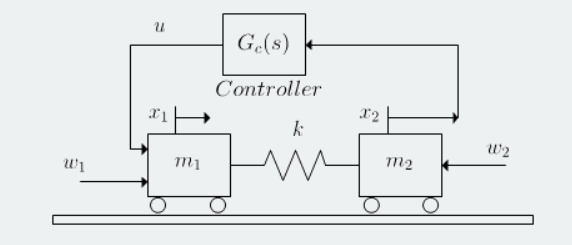
\includegraphics[width=.5\linewidth]{images/2_mass_1_spring.PNG}
    \caption{Two-mass-one-spring system}
    \label{spring_sys}
\end{figure}

\noindent Below are the given definitions of matrices $A,B_1,\: and \: B_2$:

\begin{equation*}
    A = 
    \begin{bmatrix}
    0 & 0 & 1 & 0 \\
    0 & 0 & 0 & 1 \\
    -k & k & 0 & 0 \\
    k & -k & 0 & 0 \\
    \end{bmatrix}, \:
     B_1 = 
    \begin{bmatrix}
    0  \\
    0  \\
    1 \\
    0 \\
    \end{bmatrix}, \:
     B_2 = 
    \begin{bmatrix}
    0  \\
    0  \\
    0 \\
    -1 \\
    \end{bmatrix}
\end{equation*}

Matrix $A$ depends affinely on k. So by letting $k= 1.25 + \frac{3}{4}\Bar{k}$, $A$ can be further expressed as $A = A_0 + A_1 \Bar{k} A_2^T$, where $A_0$, $A_1$, and $A_2$ are constant matrices and \Bar{k} is an unknown constant in the range of [-a,a].
\begin{equation*}
    A_0= 
    \begin{bmatrix}
    0 & 0 & 1 & 0 \\
    0 & 0 & 0 & 1 \\
    -1.25 & 1.25 & 0 & 0 \\
    1.25 & -1.25 & 0 & 0 \\
    \end{bmatrix}, \:
    A_1 = 
    \begin{bmatrix}
    0  \\
    0  \\
    -\frac{\sqrt{2}}{2} \\
    \frac{\sqrt{2}}{2} \\
    \end{bmatrix}, \:
     A_2 = 
    \begin{bmatrix}
    \frac{3\sqrt{2}}{4}  \\
    -\frac{3\sqrt{2}}{4} \\
    0 \\
    0 \\
    \end{bmatrix}
\end{equation*}
Thereby when $a=1$, the spring coefficient $k$ will be in the range of [0.5, 2], which comes from the original control design specifications of the original problem. Also proposed from the original problem is a 4th order stabilizing controller $u = C_c(sI-A_c)^{-1}B_cx_2$.

\begin{equation*}
     A_c = 
    \begin{bmatrix}
    0 & -0.7195 & 1 & 0 \\
    0 & -2.9732 & 0 & 1 \\
    -2.5133 & 4.8548 & -1.7287 & -0.9616 \\
    1.0063 & -5.4097 & -0.0081 & 0.0304 \\
    \end{bmatrix}, \:
    B_c = 
    \begin{bmatrix}
    0.720  \\
    2.973 \\
    -3.37 \\
    4.419 \\
    \end{bmatrix}, \:
     C_c^T = 
    \begin{bmatrix}
    -1.506  \\
    0.494 \\
    -1.738 \\
    -0.932 \\
    \end{bmatrix}
\end{equation*}

The mass-spring control system is expressed as a block diagram in Figure \ref{block_diagram}, where $B_1$, $B_2$, and $C$ are $[0010]^T$, $[000-1]^T$ and $[0100a]$ respectively.


\begin{figure}[h]
    \centering
    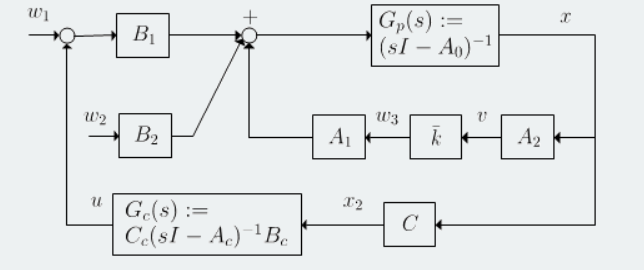
\includegraphics[width=.7\linewidth]{images/blockdiagram.PNG}
    \caption{Block diagram of the two-mass-one-spring system}
    \label{block_diagram}
\end{figure}

Next I will compute an estimate of the energy gain from $[w1, w2]$ to $x_2$. Initially estimating the gain from some external disturbance to any internal signal in the system is the best way to check for stability. A finite gain implies stability. This will all be defined in a MATLAB workspaces and will incorporate IQC$\beta$ and the MATLAB Control Systems Toolbox.

Start with initializing the abstract IQC-environment, which is necessary for the use of IQC$\beta$. Then I define the signals and design how they relate to the system. At this stage, the uncertainty is $\Bar{k}$, therefore that block will be removed and will later be replaced by set-valued functions defined by IQCs. The basic signals ($w_1$, $w_2$, $w_3$) cannot be derived from any other signals through a constant LTI transformation. They are considered external disturbances. Figure \ref{block_diagram_cont} shows the the breaking of loop found in Figure \ref{block_diagram} that described every signal as a LTI transformation of the other signals and introduced an extra basic signal $u$. We then define $x$, $x_2$, and $u_c$ as LTI transformations of basic signals including $u$. I then define the 4 basic signals ($w_1$, $w_2$, $w_3$, and $u$) as $u_c == u$. 

% insert code snippet
\begin{lstlisting}[language=MatLab]
abst_init_iqc;  %Initialize IQC-environment

%Define basic signals
w1=signal;
w2=signal;
w3=signal;
u=signal;

\end{lstlisting}

\noindent Now we relate the remaining signals ($x$, $x_2, v, u_c)$ in the system to the basic signals we just defined.

\begin{lstlisting}[language=MatLab]
%Relate basic signals to the remaining signals
x=Gp*(A1*w3+B1*(u+w1)+B2*w2);
v=transpose(A2)*x;
x2=x(2); %Also x2 = C*x
uc=Gc*x2;

\end{lstlisting}

\noindent Now we design the IQC. More explicityly we must relate $w3$ and $v$ with a set-valued function. Because $|\Bar{k}| \leq a$ we know that 
\begin{equation*}
    \int^\infty_0 (a^2 |v(t)|^2 - |w3(t)|^2)dt \geq 0
\end{equation*}
The inequality remains valid with the multiplication of any scalar larger than 0, so the following parameterized inequality holds for all pairs of ($w3. v$) which satisfy $w3 = \Bar{k}v$. In this case $M \geq 0$.

\begin{equation*}
    \int^\infty_0 M \cdot (a^2 \cdot v^2 - w_3^2)dt \geq 0
\end{equation*}

\begin{lstlisting}[language=MatLab]
%Define IQC
M=variable; %creates LMI toolbox variable 
M > 0;
v'*(aˆ2*M)*v-w3'*M*w3>0; %descibes the IQC using toolbox
u == uc;
\end{lstlisting}

\noindent Now we will execute the optimizer to estimate the L2-gain from [w1; w2] to x2. The $\text{iqc\_gain\_tbx.m}$ script will form an optimization problem which corresponds to the worst case L2-gain estimation problem. This formed as a semi-definite program (SDP). Then the LMI Control Toolbox provides the genetic SDP solver to solve the optimization problem. More explicity, the solver will choose the variable parameters $M$ and $g$ so that 
\begin{equation*}
    \int^\infty_0 (g(w_1^2 + w_2^2) - x_2^2) dt > \int_0^\infty M(a^2 \cdot v^2 - w_3^2)dt
\end{equation*}
holds for all non-zero L2 signals. The solver will also attempt to minimize $g$. 

\begin{lstlisting}[language=MatLab]
%run solver to find values for g and M
g = iqc_gain_tbx([w1;w2],x2)
value_iqc(M)
\end{lstlisting}

\noindent Below is output from Matlab Terminal.
\begin{lstlisting}
iqc_extract: processing the abst log information ... 
  Processing cst, var, and lin, counting ...
    scalar inputs:  4
    states:         26
    simple q-forms: 2
  Processing signals and quadratic forms ...
    LMI #1    size = 1    states: 0    
  iqc_extract done OK
 
iqc_gain_tbx ...
  defining the original variables ...
  defining the non-KYP LMIs ...
  defining the KYP LMIs ...
  Solving with 353 decision variables ...

 Solver for linear objective minimization under LMI constraints 

 Iterations   :    Best objective value so far 
 
     1
     2
     3
     4
     5
     6
     7
     8
     9
    10
    11
    12
    13
    14
    15
    16
    17
    18
    19
    20
    21
    22
    23
    24
* switching to QR
    25
    26
    27                 389.671972
    28                 359.120709
    29                 359.120709
    30                 334.780009
    31                 334.780009
    32                 334.780009
    33                 308.604259
    34                 308.604259
    35                 308.604259
    36                 308.604259
    37                 308.604259
    38                 308.604259
    39                 308.604259
    40                 308.604259
    41                 308.604259
    42                 308.604259
    43                 308.604259

 Result:  feasible solution
          best objective value:   308.604259
          f-radius saturation:  89.312% of R =  1.00e+09 
 Termination due to SLOW PROGRESS:
          the objective was decreased by less than 
          1.000% during the last 10 iterations.


g =

   17.5671


ans =

   94.5067
\end{lstlisting}
The final result shows 94.5067. This shows that the value of M need to achieve L2 gain estimation (g) 17.5671 is 94.5067. According to the tutorial the final result should show 117.9644, which means the value of M to obtain L2-gain estimation (g) 17.4074 is 117.9644. 


%
{\small
\bibliographystyle{ieee}
\bibliography{bibliography}
}

 \end{document}


